\documentclass[../../Main/Main.tex]{subfiles}

\begin{document}

\chapter{Role of fluctuations in critical phenomena: Ginzburg criterium, Coarse-graining and Ginzburg-Landau theory of phase transitions}

\section{Importance of fluctuations: the Ginzburg criterium}
As we have seen, the main assumption (and the most important problem) of mean field theories is that the fluctuations of the order parameter are completely neglected in the computation of the partition function \( Z \); this approximation breaks down in the neighbourhoods of critical points, where as we have seen in long range correlations the correlation length becomes comparable with the size of the system:
\begin{equation*}
   \xi \overset{T \rightarrow T_c}{\sim } \abs{T-T_c}^{-\nu }
\end{equation*}
 What we would now like to do is to include these fluctuations in a mean field theoretical framework; this will lead to the so called Ginzburg-Landau theory.

Overall, mean field is not a very good approximation in proximity of the critical point, and the question is: how bad is the mean field approximation in proximity of it?
As a first approach we can try to estimate how big is the error we make in mean field theories neglecting the fluctuations of the order parameter near a critical point, so that we can understand under which conditions mean field theories are actually a good approximations.

To make things explicit, let us use the Ising model as a base for our considerations. We have seen in Weiss mean field theory for the Ising model that the Weiss mean field theory for the Ising model is based on the assumption that
\begin{equation*}
  \expval{S_i S_j} \overset{MF}{\longrightarrow } \expval{S_i} \expval{S_j}
\end{equation*}
 i.e. that the spins are statistically independent; therefore, a possible estimate of the error dor each pair of spin \( (S_i,S_j) \) made with this assumption can be:
\begin{equation}
  E_{ij} = \frac{ \abs{\expval{S_i S_j}  - \expval{S_i} \expval{S_j}}   }{\expval{S_i}\expval{S_j}  }
\end{equation}
The numerator of \(   E_{ij}  \) is, by definition, the two-point connected correlation function:
\begin{equation}
  G_c (i,j) \equiv \expval{S_i S_j} - \expval{S_i} \expval{S_j} = \expval{(S_i -\expval{S_i} )(S_j - \expval{S_j} )}
\end{equation}
Assuming \emph{translational invariance}, we have
\begin{equation*}
  G_c (i,j) \rightarrow G_c \qty(\abs{\va{r}_i - \va{r}_j} ) \rightarrow G_c (r)
\end{equation*}
In order to compute \( G_c (r) \) we cannot assume omogeneity since \( \expval{S_i} = \expval{S_j} = m   \). It implies that \( G_c = 0 \) identically, and if we want to compute the error in the mean field, is always zero. Therefore, in order to have non-null correlation functions we need that the system exhibits some kind of inhomogeneity, not necessarily due to thermal fluctuations. In fact, the connected correlation function \( G_c \)  describes not only the spatial extension of the fluctuations of the order parameter, but also, through the linear response theory, the way in which \( m \) varies in space in response to an external inhomogeneous magnetic field.  Within a mean field theory this is the  only way to compute \( G_c \)! Let us see this explicitly. We know that from the partition function of the Ising model in an inhomogeneous external field \( \va{H}_i \), i.e.:
\begin{equation}
  Z [H_i]= \Tr_{\{ S \} } \qty(e^{-\beta \qty(-J \sum_{\expval{ij} }^{} S_i S_j   - \sum_{i}^{} H_i S_i ) } )
\end{equation}
we have  the definition of the thermal average
\begin{equation}
  \expval{S_i} = \frac{\Tr_{\{ S \} } \qty(S_i e^{-\beta \qty(-J \sum_{\expval{ij} }^{} S_i S_j   - \sum_{i}^{} H_i S_i ) } ) }{Z[H_i]}
  = \frac{1}{\beta Z}  \pdv{Z }{H_i}  = \beta ^{-1} \pdv{\ln{Z} }{H_i}
  = -\pdv{F}{H_i}
\end{equation}
Similarly, one can show that
\begin{equation}
  \expval{S_i S_j} = \frac{\beta ^{-2}}{Z} \frac{\partial^2{Z} }{\partial{H_i} \partial{H_j}  }
\end{equation}
and thus:
\begin{equation}
\begin{split}
  G_c (i,j) & = \frac{\beta ^{-2}}{Z}  \frac{\partial^2{Z} }{\partial{H_i} \partial{H_j}  }
  - \qty(\frac{\beta ^{-1}}{Z} \pdv{Z}{H_i} ) \qty(\frac{\beta ^{-1}}{Z} \pdv{Z}{H_j} ) \\
  & = \beta ^{-2} \frac{\partial^2{\ln{Z} } }{\partial{H_i} \partial{H_j}  }
  = - \frac{\partial^2{F(\{ H_i \}  )} }{\partial{H_i} \partial{H_j}  }
\end{split}
\end{equation}
Therefore, the response in \( i \) due to a variation of \( H \) in \( j \) is
  \begin{equation*}
    \pdv{}{H_j} \expval{S_i} = \pdv{}{H_j} \qty[\beta ^{-1} \pdv{\ln{Z} }{H_i} ]  =\pdv{}{H_j} \qty[-\pdv{F}{H_i} ] =  \beta G_c (i,j)
  \end{equation*}
  so \( G_c (i,j) \) can indeed be seen as a response function.
The \emph{generating functions} are:
\begin{itemize}
\item \( Z[H_i] \): generating function of \( G(i,j) \).
\item \( \ln{Z[H_i]} = - \beta F  \): generating function of \( G_c (i,j) \).
\end{itemize}
 If we now call:
\begin{equation*}
  M = \sum_{i}^{}  \expval{S_i}
\end{equation*}
we will have
\begin{equation*}
  \pdv{M}{H_j} = \sum_{i}^{} \pdv{\expval{S_i} }{H_j} = \beta  \sum_{i}^{} G_c (i,j)
\end{equation*}
If our system is invariant under translations and subject to a uniform field, then:
\begin{equation*}
  \pdv{M}{H} = \sum_{j}^{} \pdv{M}{H_j} \pdv{H_j}{H}
  =  \beta \sum_{ij}^{} G_c (i,j)
\end{equation*}
and since  \( \chi _{T}=\partial M/\partial H \) we get:
\begin{equation}
  \chi _T = \beta \sum_{i,j}^{} G_c (i,j)
  = \beta \sum_{i,j}^{} \qty(  \expval{S_i S_j} - \expval{S_i} \expval{S_j}  )
\end{equation}
which is a version of the \emph{fluctuation-dissipation theorem}.


\subsection{Fluctuation-dissipation relation}
The fluctuation–dissipation theorem (FDT), or fluctuation–dissipation relation (FDR), is a powerful tool in statistical physics for predicting the behavior of systems that obey detailed balance. It is a general result of statistical thermodynamics that quantifies the relation between the fluctuations in a system that obeys detailed balance and the response of the system to applied perturbations.

More specifically, the fluctuation–dissipation theorem says that when there is a process that dissipates energy, turning it into heat (e.g., friction), there is a reverse process related to thermal fluctuations.

For instance, let us consider the Brownian motion: if an object is moving through a fluid, it experiences drag (air resistance or fluid resistance). Drag dissipates kinetic energy, turning it into heat. The corresponding fluctuation is Brownian motion. An object in a fluid does not sit still, but rather moves around with a small and rapidly-changing velocity, as molecules in the fluid bump into it. Brownian motion converts heat energy into kinetic energy—the reverse of drag.


Now, let us consider the partition function with an homogeneous magnetic field \( H_i = H\), \( \forall i \):
\begin{equation*}
  Z_N = \Tr_{\{ S \}  } e^{ \beta J \sum_{\expval{ij} }^{} S_i S_j + H \sum_{i}^{} S_i   }
\end{equation*}
The magnetization is thus:
\begin{equation*}
  M = \sum_{i}^{} \expval{S_i} = \frac{1}{Z} \Tr_{\{ S \}  } \sum_{i}^{} S_i   e^{ \beta J \sum_{\expval{ij} }^{} S_i S_j + H \sum_{i}^{} S_i    } = \frac{1}{\beta Z_N} \pdv{Z_N}{H}
\end{equation*}
Similarly, we have
\begin{equation*}
  \sum_{ij}^{} \expval{S_i S_j} = \frac{1}{\beta ^2 Z_N} \pdv[2]{Z_N}{H}
\end{equation*}
Recall that
\begin{equation*}
   \frac{1}{N} F =  - \frac{1}{N} k_B T \ln{Z}
\end{equation*}
Hence, the magnetic supsceptibility is:
\begin{equation*}
\begin{split}
  \chi _T & = \pdv{m}{H} = \pdv{}{H} \qty[- \frac{1}{N} \pdv{F}{H} ] = \pdv{}{H}  \qty[\frac{1}{N} k_B T \pdv{\ln{Z} }{H} ] \\
  & = \frac{1}{N} k_B T \qty[\pdv[2]{\ln{Z} }{H} ] = \frac{1}{N} k_B T \qty[\frac{1}{Z} \pdv[2]{Z}{H} - \frac{1}{Z^2} \qty(\pdv{Z}{H} )^2 ] \\
  & = \frac{1}{N \beta } \qty[\beta ^2 \sum_{ij}^{} \expval{S_i S_j}  - \beta ^2 \qty(\sum_{i}^{} \expval{S_i}  )^2   ] \\
  & = \frac{\beta }{N} \sum_{ij}^{}  G_c (i,j) = \frac{\beta }{N} \sum_{ij}^{} G_c (\va{r}_i - \va{r}_j) \\
  & = \beta \sum_{i}^{} G_c (\va{x_i})
\end{split}
\end{equation*}
where we have defined \( \va{x}_i \equiv \va{r}_i - \va{r}_j \). Therefore:
\begin{equation}
  \Rightarrow \chi _T = (a^d k_B T)^{-1} \int_{\Omega }^{} \dd[d]{\va{r}} G_c (\va{r})
\label{eq:16_7}
\end{equation}
this is the fluctuation dissipation relation.

\subsection{Computation of \( \pmb{E_{TOT}}  \)}


Let us now try to understand when the error \( E_{ij} \) done in mean field theories is negligible. 


We now consider the quantity
$$
E_{\text {tot }}=\frac{\sum_{i, j}^N\left[\left\langle s_i s_j\right\rangle-\left\langle s_i\right\rangle\left\langle s_j\right\rangle\right]}{\sum_{i, j}^N\left\langle s_i\right\rangle\left\langle s_j\right\rangle}
$$

Since $G_c(i, j) \equiv\left\langle s_i s_j\right\rangle-\left\langle s_i\right\rangle\left\langle s_j\right\rangle$
$$
\begin{aligned}
E_{t o t} & =\frac{\sum_{i j}^N G_c(i, j)}{\sum_{i j}^N\left\langle s_i\right\rangle\left\langle s_j\right\rangle}=\frac{{N} \sum_i G_c\left(\bar{x}_i\right)}{\sum_{i j}\left\langle s_i\right\rangle\left\langle s_j\right\rangle} \\
& =N \frac{\sum_i G_c\left(\bar{x}_i\right)}{\sum_{_{ij}}\left\langle s_i\right\rangle\left\langle s_j\right\rangle} \quad \bar{x}_i \equiv \vec{r}_i-\bar{r}_0
\end{aligned}
$$
Given $\xi \Rightarrow$ we know that for $\left|\bar{x}_i\right|>\xi \quad G_c\left(\left|\bar{x}_i\right|\right)$ is $\sim 0$
$$
\Rightarrow \sum_i G_c\left(\bar{x}_i\right) \sim \int_{V_{\xi}} d \vec{x} G_c(|\vec{x}|)
$$
$V_\xi$ : region where $G_c(|\vec{x}|) \neq 0$

Inside this region we can assume that, if  $T < T_C$
$$
\Rightarrow \exists\,\, \eta(r)=\eta^* \neq 0 \text { (uniform) }
$$
So inside $V_{\xi}\left\langle s_i\right\rangle=\left\langle s_j\right\rangle=\eta^*$ and finally
$$\avg{s_{i}} \avg{s_{j}} \approx (\eta^{*})^{2}$$
So we get that
$$E_{TOT} = \frac{{N} \sum_i G_c\left(\bar{x}_i\right)}{\sum_{i j}\left\langle s_i\right\rangle\left\langle s_j\right\rangle} \approx \frac{N\int _{V_\xi}G_{c}(\mid \vec{x}\mid) \, d^{D}x}{N\int _{V_\xi}(\eta^{*})^{2} \, d^{D}x} $$



Now, in other words, if we formulate a mean field theory for a system we will make the error \( E_{ij} \)  in the region where correlations are relevant, namely if \( \abs{\va{r}}  \) is the distance between two points of the system the error is made for \( \abs{\va{r}} \leq \xi  \), with \( \xi  \) the correlation length.  The total relative error is the \( E_R (r)\) integrated over the region of radius \(  \abs{\va{r}} \le \xi  \), i.e. where correlations are not negligible:
\begin{equation}
  E_{TOT} = \frac{\int_{\abs{\va{r}} \le \xi  }^{} G_c (r) \dd[d]{\va{r}}  }{\int_{ \abs{\va{r}} \le \xi  }^{} \expval{S_i} \expval{S_j}  \dd[d]{\va{r}} }
\end{equation}
where we have called \( d \) the dimensionality of our system.
Supposing \( T<T_c \), so that the order parameter \( \eta  \)  is non null, i.e.  \( \eta (r) = \eta \neq 0 \), we have:
\begin{equation*}
   \expval{S_i} \expval{S_j} \approx \eta ^2
\end{equation*}
is uniform in the region \( \abs{\va{r}} < \xi   \). Hence, our mean field theory will be a good approximation if \( E_{TOT} \ll 1 \):
\begin{equation}
  E_{TOT} \sim \frac{\int_{\abs{\va{r}} \le \xi  }^{} G_c (\va{r}) \dd[D]{\va{r}}  }{\int_{ \abs{\va{r}} \le \xi  }^{ } \eta ^2 \dd[D]{\va{r}}  } \ll 1
  \label{eq:16_2}
\end{equation}
known as Ginzburg criterion. If it is satisfied, then the mean field theory is a valid approximation.


\subsection{Estimation of \( \pmb{E_{TOT}} \) as \( \pmb{t \rightarrow 0^-} \)  }
In order to express Eq.\eqref{eq:16_2} in a useful fashion, let us write it in terms of critical exponents; using also the version we have just found of the fluctuation-dissipation theorem (Eq.\eqref{eq:16_7}) we get (supposing our system is continuous) that the numerator of Eq.\eqref{eq:16_2} can be approximated as
\begin{equation*}
  \int_{\abs{\va{r}} \le \xi }^{} G_c (r)\dd[d]{r} \overset{\substack{ \text{fluctuation} \\  \text{dissipation} } }{\sim } k_B T_c \chi _T \sim t^{-\gamma  }
\end{equation*}
On the other hand, the denominator can be approximated as
\begin{equation*}
  \int_{\abs{\va{r}} \le \xi }^{} \eta ^2 \dd[d]{r} \sim \xi ^d \abs{t}^{2 \beta } \sim t^{2 \beta - \nu d}
\end{equation*}
 Therefore, the Ginzburg criterion can be reformulated as:
\begin{equation*}
  E_{TOT} \overset{t \rightarrow 0^-}{\sim } t^{- \gamma + \nu d - 2 \beta  } \ll 1
\end{equation*}
and in the limit \( t \rightarrow 0^- \) this is possible only if \(  - \gamma + \nu d - 2 \beta >0  \), i.e.:
\begin{empheq}[box=\myyellowbox]{equation}
  d > \frac{\gamma + 2 \beta  }{\nu } \equiv d_c
\end{empheq}
This means that Ginzburg criterion allows us to determine the \emph{upper critical dimension} \( d_c \) of a system, namely the dimension above which mean field theories are good approximations. Let us consider three different cases:
\begin{itemize}
\item Case \( d < d_c \): fluctuations are relevant and mean field is no a good approximation.
\item Case \( d > d_c \): fluctuations are less important and mean field describes properly the critical point.
\item Case \( d = d_c \): mean field critical exponents ok but strong correction to the scaling expected. For a Ising-like systems (in the mean field) we have
\begin{equation*}
  \beta = \frac{1}{2}, \quad \gamma =1 \quad \Rightarrow d_c = \frac{2}{\nu}
\end{equation*}
In order to compute \( d_c \) we need to compute \( \nu  \) withing the mean field approximation. Let us note that since it depends on the critical exponents, the upper critical dimension \( d_c \)  ultimately depends on the universality class of the system considered; furthermore, in order to actually be able to compute \( d_c \)  we must generalize Landau theory to systems with spatial inhomogeneities so that we are able to compute the critical exponent \( \nu  \).

\begin{remark}
Remind that within the mean field theory the \( \nu  \) exponent it is not defined. In fact, the \( \nu  \) exponent define the divergence of the correlation length, but in the mean field we neglet correlation between fluctuations.

We have \( \nu _{MF} = 1/2 \), hence the upper critical dimension for the mean field is \( d>4 \).
\end{remark}


\end{itemize}


\section{Spatial Variations: coarse graining procedure and the Ginzburg-Landau Model}
Since in proximity of the critical point the correlation length \( \xi  \) diverges, there is no point in which we can see small scales. It is convenient to rewrite the microscopic partition function as an effective partition function obtained by integrating out the degrees of freedom over regions of linear size \( l \gg a \) but still \( l \ll \xi  \). Indeed, a possible way to overcome the limitations of mean field theories can be the following: we could regard the profile of the order parameter \( m (\va{r}) \) to be the "degree of freedom" of our system and compute the partition function as a functional integral; in other words from the microscopic configuration of our system we can obtain \( m (\va{r}) \) with a \emph{coarse graining procedure} (we will immediately see what we mean by this) and then determine \( Z \) as a trace over all the possible configurations of our system, i.e. over all the possible forms of \( m(\va{r}) \):
%This \emph{coarse graining procedure} is formally given by
\begin{equation}
  Z = \Tr_{\{ S \}  } e^{- \beta \mathcal{H} [ \{ S \}  ]}
  = \int_{}^{} \mathcal{D}{\qty[m(\va{r})] } \qty[\sum_{ \substack{ \{ S \} \\ \text{compatible with the} \\ \text{profile } m(\va{r})}   }^{} e^{- \beta \mathcal{H} [ \{ S \}  ]] } ]
\end{equation}
where we traced over all the possible microscopic configurations \( \{ S \}   \) compatible with the order parameter profile \( m(\va{r}) \).
Let us define the effective Hamiltonian \( \mathcal{H}_{eff} \):
\begin{equation}
\sum_{ \substack{ \{ S \} \\ \text{compatible with the} \\ \text{profile } m(\va{r})}   }^{} e^ {- \beta \mathcal{H} [ \{ S \}  ]}
= e^{-\beta \mathcal{H}_{eff} (m (\va{r}))}
\label{eq:17_7}
\end{equation}
How, in pratice, can we perform the coarse graining procedure and obtain \( \mathcal{H}_{eff} \)?
We therefore must understand how to determine \( m(\va{r}) \); the idea of coarse graining procedures is the following: for a given microscopic configuration \( \{ S \}   \)  we average the order parameter \( m(\va{r}) \)  over sufficiently wide "blocks", i.e. portions of the system with linear dimension \( l \) much greater than its microscopic scale, which we call \( a \) (in the case of the Ising model, for example, \( a \)  can be taken as the lattice constant), but still microscopic and in particular much smaller than the correlation length \( \xi \), so that the order parameter is uniform in every block. In other words, coarse graining a system means dividing it into cells of linear dimension \( l \),  with \( l \) such that:
\begin{equation}
  a \ll l \ll \xi (T) < L
  \label{eq:17_1}
\end{equation}
(\( L \)  being the linear dimension of our system) and averaging the order parameter  \( m(\va{r}) \).  This way we can obtain an expression for \( m(\va{r}) \) (since \( l \) is anyway microscopic with respect to the size of the system, so we can regard  \( \va{r} \) as a continuous variable).

\begin{remark}
Hence, we partition the configurations according to the magnetization profile. For example, if we have a configuration with half spin up and half down, we obtain a profile with 1 and -1.
\end{remark}

\section{Coarse graining procedure for the Ising model}
To make things more clear, let us see how the coarse graining procedure works for the Ising model. For instance, see the two dimensional system represented in Figure \ref{fig:17_1}, where we have many spins in each square in which the system is divided.

\begin{figure}[H]
\centering
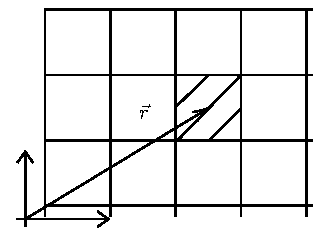
\includegraphics[width=0.5\textwidth]{./img/1.pdf}
\caption{\label{fig:17_1} Two dimensional system divided into cells with a huge number of spins.}
\end{figure}

If we call \( m_i = \expval{S_i}  \) the local magnetization at the \( i \)-th  and \( d \) the dimensionality of the system, once we have choosen the linear dimension \( l \), every "block" will have volume \( l^d \); we replace what it is inside every block of the system centered in \( \va{r} \), with the coarse grained magnetization:
\begin{equation}
  m_l (\va{r}) = \frac{1}{N_l} \sum_{i \in \va{r}}^{} S_i
\end{equation}
where \( N_l = (l/a)^d \) is the number of spins in each cell.

\begin{remark}
Since close to the critical point \( T_c \), we have that the correlation length diverges \( \xi \gg a \), we can always choose \( l \ll \xi  \) but still \( l \gg a \) such that the number \( N_l \) is large enough.
In this way, \( m(\va{r}) \) can be made to be a regular function of \( \va{r} \).
\end{remark}

Moreover, since it has been built as an average, \( m_l (\va{r}) \) does not fluctuate much on microscopic scales but varies smoothly in space. Of course, in general we need to specify \( l \) in order to determine \( m_l \), but the coarse graining procedure we are applying will be useful only if the final results are independent of \( l \)  (at least in the spatial scales considered).

\begin{remark}
In the reciprocal space (Fourier transform), the bound in Eq.\eqref{eq:17_1} implies the following cut off on the wave vector \( \va{q} \):
\begin{equation*}
  \abs{\va{q}} > \Lambda  = l^{-1}
\end{equation*}
Hence, this theory cannot develop ultraviolet divergences!
\end{remark}

We now must express the partition function in terms of \( m_l (\va{r}) \):
\begin{equation*}
  Z = \sum_{m_l (\va{r})}^{} \qty(\sum_{ \substack{ \{ S \} \\ \text{compatible with the} \\ \text{profile } m(\va{r})}   }^{} e^{-\beta \mathcal{H} ( \{ S \}  )}   )
 = \sum_{m_l(\va{r})}^{} e^{-\beta \mathcal{H}_{eff} [m(\va{r})]}
\end{equation*}
If \( m(\va{r}) \) is regular, the sum converges to a functional integral:
\begin{equation}
   Z_{GL} = \int_{}^{} \mathcal{D}  \qty[m_l (\va{r})]  e^{-\beta \mathcal{H}_{eff}[m(\va{r})]}
   \label{eq:17_8}
\end{equation}
so we must compute \( \mathcal{H}_{eff} [m(\va{r})] \).
First let us notice that Eq.\eqref{eq:17_7}:
\begin{equation*}
  \sum_{ \substack{ \{ S \} \\ \text{compatible with the} \\ \text{profile } m(\va{r})}   }^{} e^ {- \beta \mathcal{H} [ \{ S \}  ]}
  = e^{-\beta \mathcal{H}_{eff} (m (\va{r}))}
\end{equation*}
is proportional to the probability that the system displays a configuration with a profile \( m_l (\va{r}) \).

\subsection{Computation of \( \pmb{\mathcal{H}_{eff} [m(\va{r})]}\)}
 Since we now have a system made up of "blocks" this effective Hamiltonian will be composed of two parts: a bulk component relative to the single blocks and an interface component relative to the interaction between the blocks; let us consider them individually.

 \begin{itemize}
 \item \textbf{Bulk component}: suppose that every block of volume \( l^d \)  is separate from the rest of the system; inside every one of them the magnetization is uniform (since the linear dimension of the blocks is much smaller than the correlation length  \( l \ll \xi  \)), so we can use Landau theory for uniform systems. In the case of the Ising model, it led to the free energy:
\begin{equation*}
  \mathcal{L} = a t m^2 + \frac{\bar{b} }{4} m^4
\end{equation*}
The total bulk energy is thus obtained summing over all the blocks:
\begin{equation}
  \beta \mathcal{H}_{eff}^{bulk} [m] = \sum_{\va{r}}^{}  \bar{a} t m^2 (\va{r})+ \frac{\bar{b} }{2} m^4 (\va{r})
\end{equation}
Hence, the probability that the sistem displays a configuration with a profile \( m_l (\va{r}) \) is proportional to
\begin{equation}
  P^{cell} (m_l (\va{r})) \simeq e^{-\beta \mathcal{H}_{eff}^{bulk} (m (\va{r}))} = e^{ - \sum_{\va{r}}^{}  \bar{a} t m^2 (\va{r})+ \frac{\bar{b} }{2} m^4 (\va{r}) }
\end{equation}


\item \textbf{Interaction component:} we now must take into account the fact that adjacent blocks do interact. In particular, since as we have stated \( m \) does not vary much on microscopic scales, the interaction between the blocks must be such that strong variations of magnetization between neighbouring blocks is energetically unfavourable. If we call \( \va{\mu } \) a vector of magnitude \( l \) (\( \abs{\va{\mu }} =l  \)) that points from one block to a neighbouring one (see Figure \ref{fig:17_2}), the most simple analytic expression that we can guess for such a term can be a harmonic one:
\begin{equation}
  - \beta \mathcal{H}_{eff}^{int} =   \sum_{\va{r}}^{}  \sum_{\va{\mu }}^{}  \frac{\bar{k} }{2} \big( m (\va{r}+\va{\mu }) - m(\va{r})\big)^2 + O \qty( \qty(m (\va{r}+\va{\mu }) - m(\va{r}))^4 )
 \end{equation}
 (the factor \( 1/2 \) multiplying \( \bar{k}  \), just like the numeric factors multiplying \( \bar{a}  \)  and \( \bar{b}  \), have been inserted for future convenience). We can also think of this as a first approximation of a general interaction between the blocks, namely as the first terms of a Taylor expansion of the real interaction energy.

\begin{figure}[H]
\centering
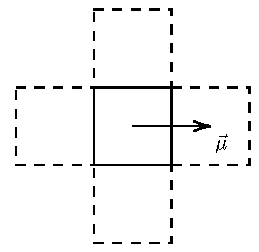
\includegraphics[width=0.3\textwidth]{./img/2.pdf}
\caption{\label{fig:17_2} Two dimensional system divided into block. The vector \( \va{\mu } \) points  from one block to a neighbouring one.}
\end{figure}

\end{itemize}

The total energy is thus obtained by summing the two terms. Now, since the linear dimension of the blocks \( l \)  is much smaller than the characteristic length \( L \) of the system we can treat \( \va{r} \)  as a continuous variable and thus substitute the sum over  \( \va{r} \) with an integral:
\begin{equation*}
  \sum_{\va{r}}^{}  \overset{\frac{l}{L} \ll 1}{\longrightarrow}   \frac{1}{l^d} \int_{}^{} \dd[d]{\va{r}}
\end{equation*}
(while the sum over \( \va{\mu } \) remains a sum, since for every \( \va{r} \)  there is only a finite number of nearest neighbours). Therefore:


\begin{itemize}
\item \textbf{Bulk component}:
\begin{equation}
  \beta \mathcal{H}_{eff}^{bulk} [m] =  \frac{1}{l^d} \int_{}^{} \qty( \bar{a} t m^2 (\va{r})+ \frac{\bar{b} }{2} m^4 (\va{r})  )  \dd[d]{\va{r}}
\end{equation}
Thus, if we now define for the sake of simplicity:
\begin{equation*}
  a \equiv \frac{\bar{a} }{l^d}, \quad b \equiv \frac{\bar{b} }{l^d}
\end{equation*}
we will have:
\begin{equation*}
  \beta \mathcal{H}_{eff}^{bulk} [m] = \int_{}^{} \qty( a t m^2 (\va{r})+ \frac{b }{2} m^4 (\va{r})  )  \dd[d]{\va{r}}
\end{equation*}


\item \textbf{Interaction component:}
\begin{equation}
  - \beta \mathcal{H}_{eff}^{int} =   \frac{1}{l^d} \int_{}^{}  \sum_{\va{\mu }}^{}  \frac{\bar{k} }{2} \big( m (\va{r}+\va{\mu }) - m(\va{r})\big)^2  \dd[d]{\va{r}}
 \end{equation}
 Keeping in mind that \( \abs{\va{\mu }}  = l \), the interaction term can be rewritten in terms of \( \va{\grad } m\):
\begin{equation*}
\begin{split}
\frac{1}{l^D} \int_{}^{}  \sum_{\va{\mu }}^{}  \frac{\bar{k} }{2} \big( m (\va{r}+\va{\mu }) - m(\va{r})\big)^2  \dd[d]{\va{r}} & = \frac{1}{l^{d-2}} \int_{}^{}
\frac{\bar{k} }{2} \sum_{\va{\mu }}^{}  \qty(\frac{m (\va{r}+\va{\mu }) - m(\va{r})}{l})^2 \dd[d]{\va{r}} \\
& = \frac{\bar{k} }{2l^{d-2}} \int_{}^{}
\sum_{\va{\mu }}^{}  \qty(\pdv{m}{ \chi  _ \mu } )^2 \dd[d]{\va{r}} \\
& \overset{\frac{a}{L} \ll \frac{l}{L} \ll 1}{\longrightarrow }  \int_{}^{}   \frac{k }{2} \qty(\va{\grad } m)^2  \dd[d]{\va{r}}
\end{split}
\end{equation*}
where we have called \( \chi _{\mu } \)  the components of \( \va{\mu } \) and we have rescaled the elastic constant by \( l^{d-2} \):
\begin{equation*}
  k \equiv  \frac{ \bar{k} }{l^{d-2}}
\end{equation*}
In this way the result is indipendent on \( l \).


\item \textbf{Total energy:}
\begin{equation}
  \beta \mathcal{H}_{eff} [m] = \int_{}^{}  \qty[a t m^2 (\va{r}) + \frac{b}{2} m^4 (\va{r}) + \frac{k}{2} \qty(\va{\grad } m (\va{r}))^2] \dd[d]{\va{r}}
\end{equation}
\end{itemize}

Therefore, the (functional) partition function of the system will be as in Eq.\eqref{eq:17_8}:
\begin{equation}
  Z_{GL} = \int_{}^{} \mathcal{D} \qty[m(\va{r})]   e^{ -\beta \mathcal{H}_{eff} [m(\va{r})]}
   = \int_{}^{} \mathcal{D} \qty[m(\va{r})]  e^{-   \int_{}^{}  \qty[a t m^2 (\va{r}) + \frac{b}{2} m^4 (\va{r}) + \frac{k}{2} \qty(\va{\grad } m (\va{r}))^2] \dd[d]{\va{r}}   }
\end{equation}
Let us now make a couple of considerations:
\begin{itemize}
\item If \( m(\va{r}) = m \) (uniform system) the energy of the system has the same structure of the one used in Landau theory.
\item The term proportional to \(   (\va{\grad } m (\va{r}))^2 \) is completely new but we could have introduced it intuitively to a Landau-like mean field functional, since the introduction of spatial variations in the order parameter has an energetic cost which must depend on how it varies in space, i.e. it depends on the gradient of \( m \). This term can be also added directly to the Landau theory by simply assuming that, whe \( m \rightarrow m(\va{r}) \) (one has to consider an additioned energy cost due to small variation of \( m \)).

Why we take \( (\va{\grad }m)^2  \) and not something else?
The choise is first of all a consequence of the isotropy of the system (all directions are equivalent). Since the system is isotropic and \( \mathbb{Z}^2 \)-invariant, we must use combinations of derivatives that are invariant under rotations and parity, and, among all the possible combinations, \(   (\va{\grad } m (\va{r}))^2 \) is the simplest one.

\end{itemize}

\begin{remark}
Let us consider the cases in which  \( m \rightarrow \va{m} \) (\( O(n) \) models); we have:
\begin{equation*}
  (\grad \va{m})^2 = \sum_{i=1}^{n} \sum_{\alpha =1}^{d}  \partial_ \alpha {m_i} \partial_ \alpha   {m_i}
\end{equation*}
Higher order terms are:
\begin{equation*}
  \qty(\grad ^2 \va{m})^2 =  \sum_{i=1}^{n} \sum_{\alpha =1}^{d} \sum_{\beta =1}^{d}
  \qty(\partial_ \alpha \partial_ \alpha {m_i}) \qty( \partial_ \beta \partial_ \beta {m_i})
\end{equation*}
and
\begin{equation*}
  \va{m}^2 \qty(\grad  \va{m})^2 =  \sum_{i=1}^{n} \sum_{j=1}^{n} \sum_{\alpha  =1}^{d} m_i m_i \partial_ \alpha {m_j} \partial_ \alpha {m_j}
\end{equation*}
In most cases it is sufficient to consider only the lowest order term.
\end{remark}

\subsection{Magnetic non-homogeneous field}
If there is also an external magnetic field
\begin{equation*}
  \va{h} ( \va{r}) = \beta \va{H} ( \va{r})
\end{equation*}
we must add to the Hamiltonian the term (Legendre transform):
\begin{equation*}
  - \int_{}^{}  \va{h} (\va{r}) \vdot \va{m} (\va{r}) \dd[d]{\va{r}}
\end{equation*}
so that the partition function becomes:
\begin{equation}
  Z_{GL} = \int_{}^{} \mathcal{D} \qty[m(\va{r})]  e^{-   \int_{}^{}  \qty[a t m^2 (\va{r}) + \frac{b}{2} m^4 (\va{r}) + \frac{k}{2} \qty(\va{\grad } m (\va{r}))^2 -  \va{h} (\va{r}) \vdot \va{m} (\va{r}) ] \dd[d]{\va{r}}   }
\end{equation}
which is a functional of \( m(\va{r}) \)  and \( \va{h}(\va{r}) \). As usual, all the thermodynamics of the system can be obtained from  \( Z_{GL} \), provided that now we take functional derivatives instead of usual derivatives.
Moreover, the free energy functional is defined as
\begin{equation}
  F [m,h] = \int_{}^{} \dd[d]{\va{r}} \qty[a t m^2 (\va{r}) + \frac{b}{2} m^4 (\va{r}) + \frac{k}{2} (\va{\grad }  m (\va{r}))^2 - h(\va{r})m(\va{r})]
  \label{eq:17_10}
\end{equation}


\subsection{Functional derivatives}
In the calculus of variations, a field of mathematical analysis, the functional derivative relates a change in a functional to a change in a function on which the functional depends. Functionals are usually expressed in terms of an integral of functions, their arguments, and their derivatives.

\begin{definition}{Functional derivative}{}
Given a manifold \( M \)  representing (continuous/smooth) functions \( h \)  (with certain boundary conditions etc.), and a functional \( G \)  defined as \( G: M \rightarrow \R \).
The functional derivative of \( G[h] \), denoted \( \delta G/\delta h \), is defined by
\begin{equation*}
  \int_{}^{}  \frac{\delta G }{\delta h}\qty(x) \Phi  (x) \dd[]{x}
= \lim_{\varepsilon \rightarrow 0} \frac{G \qty(h  +  \varepsilon \Phi  )- G(h)}{\varepsilon }
=\qty[ \dv{}{\varepsilon }  G[ h + \varepsilon \Phi  ]]_{\varepsilon =0}
\end{equation*}
where \( \Phi  \) is an arbitrary function.
In physics, it is common to use the Dirac delta function \( \delta (x-y) \) in place of a generic test function \( \Phi (x) \), for yielding the functional derivative at the point \( y \):
\begin{equation*}
\frac{\delta G [h(x)] }{\delta h(y)}  = \lim_{\varepsilon \rightarrow 0}
\frac{G [h(x) + \varepsilon \delta (x-y) ] - G[h(x)]}{\varepsilon }
\end{equation*}
or, in many dimensions:
\begin{equation}
\frac{\delta G [h(\va{r})] }{\delta h(\va{r'})}  = \lim_{\varepsilon \rightarrow 0}
\frac{G [h(\va{r}) + \varepsilon \delta (\va{r}-\va{r}') ] - G[h(\va{r})]}{\varepsilon }
\end{equation}
\subsubsection{Properties}
Like the derivative of a function, the functional derivative satisfies the following properties, where \( F[h] \) and \( G[h] \) are functionals:
\begin{itemize}
\item Linearity:
\begin{equation*}
  {\frac  {\delta (\lambda F+\mu G)[h ]}{\delta h (x)}}=\lambda {\frac  {\delta F[h ]}{\delta h (x)}}+\mu {\frac  {\delta G[h ]}{\delta h(x)}}
\end{equation*}
where \( \lambda\), \(\mu  \) are constants.
\item Product rule:
\begin{equation*}
{\frac  {\delta (FG)[h ]}{\delta h(x)}}={\frac  {\delta F[h ]}{\delta h (x)}}G[\rho ]+F[h]{\frac  {\delta G[h ]}{\delta h (x)}}
\end{equation*}
\item Chain rules:
if \( F \)  is a functional and \( G \)  another functional, then
\begin{equation*}
  \frac{\delta F[G[h]] }{\delta h(y)}  = \int dx \eval{\frac{\delta F[G]}{\delta G(x)}}_{G = G[h]} \cdot\frac {\delta G[h](x)} {\delta h(y)}
\end{equation*}
If \( G \)  is an ordinary differentiable function (local functional) \( g \), then this reduces to:
\begin{equation*}
   {\frac {\delta F[g( h )]}{\delta h(y)}}={\frac {\delta F[g( h)]}{\delta g[h (y)]}} \dv{g(h )}{ h(y)}
\end{equation*}
\end{itemize}
\end{definition}

Let us consider some examples.

\begin{example}{Functional derivative of a function}{}
A function can be written in the form of an integral like a functional. For example,
\begin{equation*}
  f(\va{r}) \equiv F[ f ] = \int f ( \va{r}') \delta^d(\va{r}-\va{r}')\dd[d]{\va{r}'}
\end{equation*}
Since the integrand does not depend on derivatives of \( f \), the functional derivative of \(   f(\va{r})  \)  is,
\begin{equation}
  \frac{\delta f (\va{r})}{\delta f (\va{r}')} \equiv \frac{\delta F}{\delta f (\va{r}')}
  =\pdv{}{f (\va{r}')}  \qty[ f ( \va{r}') \delta^d (\va{r}-\va{r}')] =  \delta^d (\va{r}-\va{r}')
  \label{eq:17_12}
\end{equation}

\end{example}

\begin{example}{Functional derivative of interaction component of \( \pmb{\mathcal{H}_{eff} } \)}{}
The functional derivative of the interaction component of \( \mathcal{H}_{eff} [m (\va{r})]\) is
  \begin{equation}
    \frac{\delta }{\delta m (\va{r})} \qty[ \int_{}^{}  \frac{k }{2} \qty(\va{\grad } m (\va{r}'))^2  \dd[d]{\va{r}'}     ]  =- k \qty(\va{\grad } ^2 m )
    \label{eq:17_9}
  \end{equation}
\end{example}
Taking into account the result Eq.\eqref{eq:17_9}, we have:
\begin{equation}
  \expval{m(\va{r})} = - \frac{\delta F}{\delta h (\va{r})} = - \frac{\delta \ln{Z[h]} }{\delta h (\va{r})}
\end{equation}
and one can show that the magnetic suscpetibility is
\begin{equation}
\begin{split}
  \chi  (\va{r},\va{r}') & = \frac{\delta ^2 F}{\delta h(\va{r}) \delta h(\va{r}')}
  = \beta ^{-1} \frac{\delta ^2 \ln{Z[h]} }{\delta h (\va{r}) \delta h (\va{r}')}\\
  & = \beta ^{-1} \qty[ \expval{m(\va{r}) m (\va{r}')} - \expval{m (\va{r})} \expval{m(\va{r}')}  ]
   = \beta ^{-1} G_c (\va{r},\va{r}')
\end{split}
\end{equation}
The problem is again try to approximate this term as much as we can. Let us do it.



\section{Saddle point approximation: Landau theory for non-homogeneous systems}
We can now compute \( Z \), as a first approach, using the saddle point approximation; as we will see this will reproduce a Landau-like mean field theory which will also take into account the presence of inhomogeneities. In particular thanks to the new term involving \( \va{\grad } m (\va{r}) \) we will be able to compute the fluctuation correlation function and so also to determine the critical exponents \( \eta  \) and \( \nu  \). Let us recall the results previously obtained:
\begin{equation*}
  Z_{GL} = \int_{}^{} \mathcal{D} \qty[m(\va{r})]  e^{-  \beta \mathcal{H}_{eff} [m (\va{r})]   + \int_{}^{} \va{h} (\va{r}) \vdot \va{m} (\va{r})  \dd[d]{\va{r}}   }
\end{equation*}
where \( h(\va{r}) = \beta H(\va{r}) \) and
\begin{equation*}
  \beta \mathcal{H}_{eff} [m] = \int_{}^{}  \qty[a t m^2 (\va{r}) + \frac{b}{2} m^4 (\va{r}) + \frac{k}{2} \qty(\va{\grad } m (\va{r}))^2] \dd[d]{\va{r}}
\end{equation*}
Therefore we approximate \( Z \) with the leading term of the integral, i.e. we must determine the function \( m_0 \)  that maximizes the exponent, namely minimizes:
\begin{equation}
  L (m,\va{\grad } m,h) =  \beta \mathcal{H}_{eff}   - \int_{}^{} \va{h}  \vdot \va{m}  \dd[d]{\va{r}} = \int_{}^{}  \qty[a t m^2  + \frac{b}{2} m^4 + \frac{k}{2} \qty(\va{\grad } m )^2 - \va{h}  \vdot \va{m} ] \dd[d]{\va{r}}
\end{equation}
 Let \( m_0 (\va{r}) \) be the profile for which \( L (m_0 (\va{r}), h (\va{r}) ) \) is minimum, then compute \( Z_{GL} \) as
\begin{equation}
  Z_{GL} [h] \overset{\substack{ \text{saddle} \\  \text{point} } }{\simeq } Z_{GL}^0 [h] = e^{- L [m_0 (\va{r})]}
\end{equation}
In order to find the minimum \( m_0 (\va{r}) \), one has to impose the stationarity condition of the functional \( L \): % with respect to \( m \):
% \begin{equation}
%   \eval{\frac{\delta L}{\delta m}}_{m_0} = 0
%   \label{eq:17_3}
% \end{equation}
\begin{equation}
  \delta L = 0
  \label{eq:17_3}
\end{equation}
Now, let us define \( \mathfrak{h} \) the integrand of \( \beta \mathcal{H}_{eff} \):
\begin{equation*}
  \mathfrak{h} = a t m^2 + \frac{b}{2} m^4 + \frac{k}{2} (\va{\grad } m)^2
\end{equation*}
By considering \( \delta L \) with respect to the variations \( \delta m \) and \( \delta (\grad m) \), one gets the equation of state
\begin{empheq}[box=\myyellowbox]{equation}
  h (\va{r}) = - \qty[\va{\grad } \qty(\pdv{ \mathfrak{h} }{(\va{\grad }m)} ) - \pdv{\mathfrak{h} }{m}  ]
  \label{eq:17_2}
\end{empheq}
Hence, by using the definition of \( \mathfrak{h} \), we obtain the state equation:
\begin{equation}
  h (\va{r}) = - k \va{\grad } ^2 m_0 (\va{r}) + 2 a t m _0 (\va{r}) + 2 b m_0^3 (\va{r})
   \label{eq:17_4}
\end{equation}
  this is the mean field solution of the Gibbs-Landau. It is more general than the one found before, indeed it has the additional term \( \va{\grad } \).
Let us note that:
\begin{itemize}
\item If \( h= 0 \): Eq.\eqref{eq:17_2} reduces to the \emph{Euler-Lagrange equation}
\begin{equation}
  \pdv{\mathfrak{h} }{m} = \va{\grad } \qty(  \pdv{\mathfrak{h}}{(\va{\grad } m)})
  \label{eq:17_11}
\end{equation}

\item If \( h (\va{r}) = h \) (homogeneous field) and \( m_0 (\va{r})=m_0 \): Eq.\eqref{eq:17_4} reduces to the equation of state of the Landau theory of uniform systems
\begin{equation*}
  h = 2 a t m_0 + 2 b m_0 ^3
\end{equation*}

\end{itemize}

 \begin{remark}
Moreover, note that a mean field theory of systems with spatial disomogeneity can start directly by considering the free energy functional defined in Eq.\eqref{eq:17_10}:
   \begin{equation*}
     F[m,h] = \int_{}^{}  \qty[a t m^2 (\va{r}) + \frac{b}{2} m^4 (\va{r}) + \frac{k}{2} (\grad m)^2 - h (\va{r}) m(\va{r})] \dd[d]{\va{r}}
   \end{equation*}
\end{remark}





\begin{example}{Show relation \eqref{eq:17_11}}{}
Let us consider the case \( h=0 \), we want to obtain the Euler-Lagrange equation:
\begin{equation*}
  \pdv{\mathfrak{h} }{m} = \va{\grad } \qty(  \pdv{\mathfrak{h}}{(\va{\grad } m)})
\end{equation*}
In order to do that, we define
  \begin{equation*}
    L [m, \va{\grad } m,h] = \int_{}^{}  \mathcal{L} (m, \va{\grad } m,h)\dd[d]{\va{r}}
  \end{equation*}
Supposing \( h=0 \)  and looking for the variation of \( L \) with respect to the variations of \( m,\, \delta m \),  and the variation of \( \va{\grad } m, \, \delta (\va{\grad } m) \), we have:

  \begin{equation*}
  \begin{split}
  \delta L [m, \va{\grad } m,0]  &=  \int_{}^{} \mathcal{L} (m+\delta m, \va{\grad } m + \delta (\va{\grad } m))  \dd[d]{\va{r}} - \int_{}^{}  \mathcal{L} (m,\va{\grad } m) \dd[d]{\va{r}}   \\
  & = \int_{}^{}  \qty[\mathcal{L} (m+\delta m, \va{\grad } m + \delta ( \va{\grad } m)) - \mathcal{L} (m, \va{\grad } m)] \dd[d]{\va{r}} \\
  & = \int_{}^{} \qty[\pdv{\mathcal{L}}{m} \delta m +
  \mathcolorbox{red!30}{ \underset{f}{\pdv{\mathcal{L}}{(\va{\grad } m)} } \underset{g'}{\delta (\va{\grad } m) }  }
  ] \dd[d]{\va{r}}
  \end{split}
  \end{equation*}
  where in the last step we did a Taylor expansion around \( (m, \va{\grad } m) \).
  We now integrate by parts (i.e. \( \int_{}^{} f g' = fg - \int_{}^{} f'g     \)) the red term, obtaining
  \begin{equation*}
  \begin{split}
  \delta L &= \int_{}^{} \qty[\pdv{\mathcal{L}}{m} \delta m - \va{\grad } \pdv{\mathcal{L}}{(\va{\grad } m)} \delta m ] \dd[d]{\va{r}} +
  \mathcolorbox{blue!20}{\int_{}^{}  \qty[\pdv{\mathcal{L}}{\va{\grad } m} \delta m ] \dd[d]{\va{r}} }
  \\
   & = \int_{}^{}  \qty[\pdv{\mathcal{L}}{m} \delta m - \va{\grad } \pdv{\mathcal{L}}{(\va{\grad } m)} \delta m ]\dd[d]{\va{r}} + \mathcolorbox{blue!20}{\int_{V}^{}  \va{\grad } \qty[\pdv{\mathcal{L}}{\va{\grad } m} \delta m ] \dd[d]{\va{r}} }
  \end{split}
  \end{equation*}
  where for the blue term we have used the divergence theorem \( \int_{\partial{ \Omega }}^{} F = \int_{V}^{} \va{\grad } F     \). Moreover, the blue term vanishes at the boundary of the integration. Hence, we have
  \begin{equation*}
    \delta L = \int_{}^{} \delta m \qty[\pdv{\mathcal{L}}{m} - \va{\grad } \pdv{\mathcal{L}}{(\va{\grad } m)}  ]  \dd[d]{\va{r}}
  \end{equation*}

  The stationarity condition \( \delta L = 0 \) (Eq.\eqref{eq:17_3}) is true \( \forall \delta m \neq 0 \) if and only if the integrand is zero, thus we obtain the \emph{Euler-Lagrange equation}:
  \begin{equation*}
    \pdv{\mathcal{L}}{m} - \va{\grad } \qty(\pdv{\mathcal{L}}{(\va{\grad } m)} ) = 0
  \end{equation*}
  Hence, when \( h=0 \), we have \( \mathcal{L} \rightarrow  \mathfrak{h} \).

\end{example}





\section{Correlation function in the saddle point approximation for non-homogeneous systems}
\label{sec:17_1}
We can now proceed to compute the correlation function within our approximations. In order to do that, we take the (functional!) derivative of the state equation \eqref{eq:17_4} with respect to \( h (\va{r}') \). Remembering that
\begin{equation*}
  \chi _T (\va{r},\va{r}') = \frac{\delta m(\va{r})}{\delta h (\va{r}')}
\end{equation*}
and that from Eq.\eqref{eq:17_12}:
\begin{equation*}
  \frac{\delta h (\va{r})}{\delta h (\va{r}')} = \delta (\va{r}-\va{r}')
\end{equation*}
The functional derivative becomes
\begin{equation}
  \delta  (\va{r} - \va{r}')  = \frac{\delta h(\va{r})}{\delta m (\va{r})} \frac{\delta m(\va{r})}{\delta h (\va{r}')} = \qty[- k \va{\grad }^2 + 2 a t    + 6 b m_0^2 (\va{r}) ]   \chi _T (\va{r}-\va{r}')
\end{equation}
where we have assumed translational invariance (i.e. uniform systems).
Now, from fluctuation-dissipation theorem we know that:
\begin{equation*}
  G_c (\va{r}-\va{r}') = k_B T \chi _T (\va{r}-\va{r}')
\end{equation*}
so that
\begin{equation}
  \beta \qty[-k \va{\grad } ^2 + 2 a t + 6 b m_0 ^2 ] G_c (\va{r}-\va{r}') = \delta (\va{r}- \va{r}')
  \label{eq:17_5}
\end{equation}
Note that this means that the correlation function \(  G_c (\va{r}-\va{r}')\)  can be interpreted as the Green's function of the operator \( D \) written between the square brackets:
\begin{equation*}
  D \equiv - k \va{\grad } ^2 + 2 a t + 6 b m^2
\end{equation*}
the equation \eqref{eq:17_5} is also known as \emph{Fundamental Equation} and \( G_c (\va{r}- \va{r}') \)  as Fundamental Solution, or Green's function of the differential operator \( D \).

As said, in case of translationally invariant (i.e. uniform) systems, \( m \) is constant and equal to the equilibrium values given by the Landau theory for the Ising model; in particular, depending on the sign of \( t \) there are two possible situations:
% We now look for the solutions of \eqref{eq:17_5}.  We consider two cases, \( T > T_c \) and \( T < T_c \) and let \( h \rightarrow 0 \).
\begin{itemize}

\item Case \( t>0 \) (\( T > T_c \)): in this case the mean field solution is \( m (\va{r}) = m_0 = 0 \), so the last equation becomes:
\begin{equation}
  \qty(-k \grad ^2 + 2 a t ) G_c (\va{r}-\va{r}') = k_B T \delta (\va{r}-\va{r}')
  \label{eq:17_6}
\end{equation}
Defining:
\begin{equation*}
  \xi_> (t) \equiv  \qty(\frac{k}{2 a t })^{1/2}
\end{equation*}
this can be rewritten as:
\begin{equation*}
  \qty(-\grad ^2 + \xi _> ^{-2} (t)) G_c (\va{r}-\va{r}') = \frac{k_B T}{k} \delta (\va{r}-\va{r}')
\end{equation*}


\item Case \( t<0 \) (\( T < T_c \)): in this case the magnetization is:
\begin{equation*}
  m_0 = \pm \qty(-\frac{at}{b})^{1/2}
\end{equation*}
so the differential equation for \( G_c \) becomes:
\begin{equation}
  \qty(-k \grad ^2 - 4 a t ) G_c (\va{r}-\va{r}') = k_B T \delta (\va{r}-\va{r}')
\end{equation}
Defining:
\begin{equation*}
  \xi _{<} (t) \equiv \qty(- \frac{k}{4at})^{1/2}
\end{equation*}
this can be written as
\begin{equation*}
  \qty(-\grad ^2 + \xi _<^{-2} (t))G_c (\va{r}- \va{r}') = \frac{k_B T}{k} \delta (\va{r}- \va{r}')
\end{equation*}

\end{itemize}

We will shortly see that \( \xi _{>} \)  and \( \xi _{<} \)  are the expressions of the correlation length for \( T>T_c \)  and \( T<T_c \) , respectively. We can therefore see that in both cases we get:
\begin{equation}
  \xi \sim t^{-1/2} \quad \Rightarrow \nu  = \frac{1}{2}
\end{equation}
that is the mean field value of \( \nu  \)!

\begin{remark}
Since \( \nu = 1/2 \), the upper critical dimension of a critical point belonging to the Ising universality class is
\begin{equation*}
  d_c = \frac{2}{\nu } = 4
\end{equation*}
as previously anticipated.
\end{remark}

We have seen that for both the cases, \( t>0 \) and \( t<0 \),  the correlation function  can be obtained by solving the differential equation:
\begin{equation}
  \qty(- \grad ^2 + \xi ^{-2}) G_c (\va{r}-\va{r}') = \frac{k_B T}{k} \delta (\va{r}-\va{r}')
  \label{eq:17_13}
\end{equation}
which can be can be solved  with the Fourier transform and by using spherical coordinates. 


\subsection{Solution of \eqref{eq:17_13} by Fourier transform}
\label{sec:18_1}
Let us  do the Fourier transform of Eq.\eqref{eq:17_13}:
\begin{equation*}
  \qty(- \grad ^2 + \xi ^{-2} (t)) G_c (\va{r}-\va{r}') = \frac{k_B T}{k} \delta (\va{r}-\va{r}')
\end{equation*}
If we define \( \va{x} \equiv \va{r} - \va{r}' \) and we use the following convention for the Fourier transform \( \widetilde{G} (q)  \) of \( G \):
\begin{equation*}
  \widetilde{G} (q) = \int_{- \infty }^{+ \infty }  G_c ( \abs{\va{x}} ) e^{- i \va{q} \vdot \abs{\va{x}} } \dd[d]{\abs{\va{x}} }
\end{equation*}
then transforming both sides of the equation we get:
\begin{equation}
  \qty(q^2 + \xi ^{-2}) \widetilde{G} ( q ) = \frac{k_B T}{k} \quad
   \Rightarrow \widetilde{G} ( q ) = \frac{k_B T}{k} \frac{1}{q^2 + \xi ^{-2}}
\end{equation}
where \( q = \abs{\va{q}}  \).
From this last equation we can also see that when \( T=T_c \), since \( \xi \rightarrow \infty  \)  we have \( \widetilde{G} (q) \simeq \frac{1}{q^2}  \) and so performing the inverse Fourier transform one gets
\begin{equation*}
  G_c (\abs{\va{x}} ) = \abs{\va{x}}^{2-d}
\end{equation*}
from which we have that the critical exponent \( \eta  \)  is null (we will see that explicitly once we have computed \( G \)). In fact, at \( T=T_c \) we have previously defined
\begin{equation*}
  G (r) \sim \abs{\va{x}}^{2-d- \eta }
\end{equation*}
hence, in this case we have \( \eta =0 \).
 Therefore, reminding that  \( \va{x} \equiv \va{r} - \va{r}' \) we can now determine \( G (\va{x}) \)  with the Fourier antitransform:
\begin{equation}
  G (\va{x}) = \int_{}^{}   \frac{\dd[d]{\va{q}}}{(2 \pi )^d} \frac{e^{i \va{q} \vdot \va{x}} }{q^2 + \xi ^{-2}}
\end{equation}
This integral is a bit tedious to compute, and in general its result depends strongly on the dimensionality \( d \) of the system; the general approach used to solve it is to shift to spherical coordinates in \( \R^d \) and then complex integration for the remaining part, which involves \( \abs{\va{q}}  \). In order to do some explicit computations, let us consider the case \( d=3 \); we will then have:

\begin{equation*}
\begin{split}
G(\va{x}) & =   \int_{}^{}  \frac{ \dd[3]{\va{q}}}{(2 \pi )^3} \frac{e^{i \va{q} \vdot \va{x}}}{q^2 + \xi ^{-2}}  \overset{\substack{ \text{spherical} \\ \text{coordinates}} }{=}
= \frac{1}{ (2 \pi )^3} \int_{0}^{\infty }  \frac{q^2}{q^2+ \xi ^{-2}} \dd[]{q} \int_{-1}^{+1}    e^{i q \abs{\va{x}} \cos \theta  } \dd[]{(\cos \theta  )} \int_{0}^{2 \pi } \dd[]{ \varphi}
\\
 &\overset{z \equiv \cos(\theta ) }{=}  \frac{2 \pi }{(2 \pi )^3} \int_{0}^{\infty }  \frac{q^2}{q^2 + \xi ^{-2}} \dd[]{q} \qty[\frac{  e^{i q \abs{\va{x}} z } }{i q \abs{\va{x}} } ]_{-1}^{1}
 = \frac{1}{(2 \pi )^2 \abs{\va{x}} } \int_{0}^{\infty } \frac{q \sin(q \abs{\va{x}} ) }{q^2 + \xi ^{-2}} \dd[]{q}
\end{split}
\end{equation*}
This last integral can be computed, using the residue theorem, extending it to the complex plane:
\begin{equation*}
  I = \int_{0}^{\infty } \frac{q \sin(q \abs{\va{x}} ) }{q^2 + \xi ^{-2}} \dd[]{q}
  = \frac{1}{2} \int_{- \infty }^{+ \infty } \frac{q \sin(q \abs{\va{x}} ) }{q^2 + \xi ^{-2}} \dd[]{q}
  = \frac{1}{2} \Im \oint \frac{z e^{i z \abs{\va{x}} } }{\qty(z^2 + \xi ^{-2}) } \dd[]{z}
\end{equation*}
There are two poles at \( z_P = \pm i \xi ^{-1} \); we choose as the contour of integration \( \gamma   \) which contains only the pole at \( +i \xi ^{-1} \) (see Figure \ref{fig:18_1}) and so using the residue theorem we will have:
\begin{equation*}
I  =
\frac{1}{2}  \Im \oint_\gamma \frac{z e^{i z \abs{\va{x}} } }{ \qty(z + i \xi ^{-1}) \qty(z - i \xi ^{-1})  } \dd[]{z}
 \overset{\substack{ \text{residue} \\  \text{theorem} } }{=}  \frac{1}{2} \Im \qty[2 \pi  i \text{Res} (i \xi ^{-1})]
\end{equation*}
\begin{figure}[H]
\centering
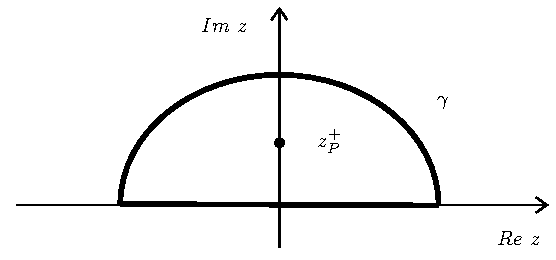
\includegraphics[width=0.6\textwidth]{./img/1__1.pdf}
\caption{\label{fig:18_1} Positive integration contour \( \gamma   \) in the complex plane for the integral \( I \). It contains only the pole at \( +i \xi ^{-1} \).}
\end{figure}

Since,
\begin{equation*}
  \text{Res} (i \xi ^{-1}) = \frac{i \xi ^{-1} e^{- \xi ^{-1} \abs{\va{x}} } }{2 i \xi ^{-1}} = \frac{e^{-\abs{\va{x}}/\xi  } }{2}
\end{equation*}
we obtain
\begin{equation}
   I = \frac{1}{2} \Im \qty[2 \pi  i \text{Res} (i \xi ^{-1})] = \frac{\pi }{2} e^{- \abs{\va{x}} /\xi }
\end{equation}
Therefore, in the end we have:H
\begin{empheq}[box=\myyellowbox]{equation}
   G ( \abs{\va{x}} ) = \frac{1}{8 \pi } \frac{e^{- \abs{\va{x}}/\xi } }{\abs{\va{x}} }
\end{empheq}
We see now clearly that the correlation function has indeed an exponential behaviour (as we have stated also in long range correlations) and that \( \xi  \)  is really the correlation length; furthermore, \( G(\va{x}) \sim 1/ \abs{\va{x}}  \) and from the definition of the exponent \( \eta  \)  we have \(  G(\va{x}) \sim 1/ \abs{\va{x}}^{d-2 + \eta } \),  so since \( d=3 \)  we indeed have \( \eta =0 \).

One can also solve the equation for \( G(\va{r}- \va{r}') \)   by using the spherical coordinates and use the Bessel functions.



Therefore, we have seen that for the Ising model \( \nu = 1/2 \). If we also consider the values of the other critical exponents we see that the upper critical dimension for this model is \( d=4 \). In other words, mean field theories are actually good approximations for the Ising model if \( d \geq 4 \). We will later see some other confirmations of this fact.





\section{Including fluctuations at the Gaussian level (non interacting fields)}
Until now even if we have introduced Ginzburg-Landau theory we are still neglecting the effects of the fluctuations since we are regarding the mean field theory approximation for non-homogeneous systems as a saddle point approximation of a more general theory; in other words, since we are approximating
\begin{equation*}
  Z_{GL} [h] \overset{\substack{ \text{saddle} \\  \text{point} } }{\simeq } Z_{GL}^0 [h] = e^{- L [m_0 (\va{r})]}
\end{equation*}
we are still regarding the magnetization \( m \) as non fluctuating over the system. In order to include the fluctuations we must do more and go further the simple saddle point approximation. The simplest way we can include fluctuations in our description is expanding \( Z \) expressed as a functional integral around the stationary solution and keeping only quadratic terms; this means that we are considering fluctuations that follow a normal distribution around the stationary value. The important thing to note, however, is that in this approximation these fluctuations are independent, i.e. they do not interact with each other. As we will see, with this assumption the values of some critical exponents will differ from the "usual" ones predicted by mean field theories.

Hence, let us introduce fluctuations at the Gaussian level. Consider consider \( h=0 \) and \( m_0 (\va{r})= m_0 \) be the solution of the saddle point approximation. Let us expand the general expression
\begin{equation*}
  \beta \mathcal{H}_{eff}  [m (\va{r})] = \int_{}^{}  \qty( a t m^2 + \frac{b}{2} m^4 + \frac{k}{2} \qty(\va{\grad } m)^2 ) \dd[d]{\va{r}}
\end{equation*}
by using
\begin{equation*}
  m(\va{r}) = m_0 + \delta m(\va{r})
\end{equation*}
If we assumed that the fluctuations \(  \delta m(\va{r})\) are small, we would obtain:
\begin{subequations}
\begin{align*}
   \qty(\grad m)^2 &= \qty(\grad \qty(m_0 + \delta m) )^2 = \qty(\grad \qty(\delta m) )^2  \\
     m^2 &= m_0^2 + 2 m_0 \delta m + \qty(\delta m)^2 \\
     m^4 &= m_0^4 + 4 m_0^3 \delta m + 6 m_0^2 (\delta m)^2 + 4 m_0 \delta m^3 + (\delta m)^4
\end{align*}
\end{subequations}
Hence, we have
\begin{equation}
  \beta \mathcal{H}_{eff} = V \underbrace{ \qty(a t m_0^2 + \frac{b}{2} m_0^4) }_{A_0}
  + \int_{}^{} \qty(\frac{k}{2}\qty( \va{\grad } (\delta m))^2 + \qty(a t + 3 b m_0^2)\delta  m^2 + 2 b m_0 \delta m^3 + \frac{b}{2} \delta m^4 )\dd[d]{\va{r}}
  \label{eq:18_10}
\end{equation}
where \( V \) is the volume of the system and the term proportional to \( \delta m \),  \( \qty( 2 a t m_0  +  2b m_0^3 )  \), is zero since \( m_0 \) is the solution of the extremal condition (\( m_0 \) is the stationary solution)
\begin{equation*}
  \eval{\frac{\delta \mathcal{H}_{eff}}{\delta m}}_{m=m_0} = 0
\end{equation*}
For simplicity let us first consider \( T>T_c \); in this case, we know that \( m_0 = 0 \) and hence,
\begin{equation*}
   m (\va{r}) = m_0 + \delta m(\va{r}) = \delta m (\va{r})
\end{equation*}
We have also \( A_0 =0 \),  \( 3bm_0^2 \delta m^2 = 0 \) and \( 2 b m_0 \delta m^3 = 0 \). Taking all of this into account, we obtain:
\begin{equation*}
  \beta \mathcal{H}_{eff}^{T>T_c} (\delta m)= \int_{}^{} \dd[d]{\va{r}} \qty(\frac{k}{2} \qty(\va{\grad }\delta m)^2 + a t (\delta m)^2 + \frac{b}{2} (\delta m)^4 )
\end{equation*}
The Gaussian approximation consists in neglecting the quartic term \( (\delta m)^4 \), hence we finally obtain:
\begin{equation}
    \beta \mathcal{H}_{eff}^{G,T>T_c} (\delta m) \simeq  \int_{}^{} \dd[d]{\va{r}} \qty(\frac{k}{2} \qty( \va{\grad } \delta m)^2 + a t (\delta m)^2 )
    \label{eq:18_4}
\end{equation}
\begin{remark}
It is important to understand that these are fluctuations with respect to the solution \( m_0 \).
\end{remark}

In order to compute this integral it is more convenient to shift to Fourier space.




\subsection{Gaussian approximation for the Ising model in Ginzburg-Landau theory}
For simplicity, consider the case \( T>T_c \); now, let us compute the partition function
\begin{equation}
  Z_{G} (\delta m) = \int_{}^{} \mathcal{D} \qty[\delta m] e^{- \int_{}^{} \dd[d]{r} \qty(\frac{k}{2} \qty(\grad \delta m)^2 + a t (\delta m)^2  )  }
 \end{equation}
 in the Fourier space.
 Let us make some remarks on what happens when we apply Fourier transformations in this case. If our system is enclosed in a cubic box of volume \( V = L^d \) (with periodic boundary conditions), we can define the Fourier components of the magnetization as:
 \begin{equation}
   \delta m_{\va{k}} = \int_{V}^{}  \delta m (\va{r}) e^{-i \va{k} \vdot \va{r} }\dd[d]{\va{r}}
 \end{equation}
 where \( \va{k} = k_1, \dots, k_d = \frac{2 \pi  \va{n} }{L}\) with \( k_ \alpha = \frac{2 \pi }{L} n_ \alpha  \) and \( n_ \alpha  = 0 , \pm 1, \dots \). We can therefore expand the magnetization in a Fourier series:
 \begin{equation}
   \delta m (\va{r}) = \frac{1}{V} \sum_{\va{k}}  e^{i \va{k}\vdot \va{r}} (\delta m_{\va{k}})
 \end{equation}
 Substituting this expression of \( m \) in \( \delta m_{\va{k}} \) we obtain an integral representation for the Kronecker delta; in fact:
$$\delta m_{\vec{k}} = \int_{V} \delta m(\vec{r}) e^{-i\vec{k}\cdot \vec{r}} \, d^{D}\vec{r} $$
and $\vec{k} = (k_{1},\dots,k_{D}) = \frac{2\pi \vec{n}}{L}$
and this is true only if:
\begin{equation*}
  \frac{1}{V} \int_{V}^{} e^{i(\va{k}-\va{k}')\vdot \va{r}} \dd[d]{\va{r}} = \delta _{\va{k},\va{k}'} \quad \Rightarrow   \int_{V}^{} e^{i(\va{k}-\va{k}')\vdot \va{r}} \dd[d]{\va{r}} = V \delta _{\va{k},\va{k}'}
\end{equation*}
Let us now make an observations; since \( \delta m (\va{r}) \in \R \) (is real) we have that
\begin{equation*}
  \delta m^*_{\va{k}} =  \delta m_{-\va{k}}
\end{equation*}


\subsubsection{Useful relations}
\begin{itemize}
\item Sometimes it is useful to convert the sum over \( \va{k} \) by an integral by using the density of states in the \( \va{k} \) space that is \( V/(2 \pi )^d \), hence one useful relation is
\begin{empheq}[box=\myyellowbox]{equation}
  \sum_{\va{k}}^{} \rightarrow \frac{V}{( 2 \pi )^d} \int_{\R^d}^{} \dd[d]{\va{k}}
  \label{eq:18_3}
\end{empheq}

\item From the relation Eq.\eqref{eq:18_3}, we have:
\begin{equation*}
  \frac{1}{V} \sum_{\va{k}}^{} e^{i \va{k} (\va{r}-\va{r}')}  \rightarrow \frac{1}{\cancel{V} } \frac{\cancel{V} }{(2 \pi )^d} \int_{\R^D}^{} \dd[d]{\va{k}} e^{i \va{k} (\va{r}-\va{r}')}
     = \delta (\va{r}- \va{r}')
\end{equation*}
Hence, another useful relation is:
\begin{empheq}[box=\myyellowbox]{equation}
  \frac{1}{V} \sum_{\va{k}}^{} e^{i \va{k} (\va{r}-\va{r}')} \rightarrow \delta (\va{r}-\va{r}')
\end{empheq}

\item As previously shown, by inserting \( m(\va{r}) \) into the expression for \( m_{\va{k}} \)
\begin{equation*}
  m (\va{r}) = \frac{1}{V} \sum_{\va{k}}^{} e^{i \va{k}' \va{r}} m_{\va{k}},
  \qquad   m_{\va{k}} = \int_{V}^{} m (\va{r}) e^{- i \va{k} \vdot \va{r}}  \dd[d]{\va{r}}
\end{equation*}
one gets
\begin{empheq}[box=\myyellowbox]{equation}
 \int_{V}^{}  e^{i (\va{k} - \va{k}') \vdot  \va{r}} \dd[d]{\va{r}} = V \delta _{\va{k}\va{k}'}
  \label{eq:18_1}
\end{empheq}

\item Finally, since
\begin{equation*}
  \int_{V}^{}  e^{i (\va{k}-\va{k}') \vdot \va{r}} \dd[d]{\va{r}} =   V \delta _{\va{k} \va{k}'}  \overset{V \rightarrow \infty }{\longrightarrow  } (2 \pi )^d \delta (\va{k}-\va{k}')
\end{equation*}
We get the last useful relation:
\begin{empheq}[box=\myyellowbox]{equation}
  V \delta _{\va{k} \va{k}'} \overset{V \rightarrow \infty }{\longrightarrow  } (2 \pi )^d \delta (\va{k} - \va{k}')
  \label{eq:18_5}
\end{empheq}

\end{itemize}

\begin{remark}
Our coarse graining procedure is based on the construction of blocks which have a linear dimension that cannot be smaller than \( a \), the characteristic microscopic length of the system; this means that not all the \( \va{k} \)  are allowed, and in particular we must have
\begin{equation*}
\abs{\va{k}} \le \frac{\pi }{a} = \Lambda
\end{equation*}
It is the ultraviolet cut-off!
\end{remark}



\subsubsection{Gaussian Hamiltonian in Fourier space}
We want to compute Eq.\eqref{eq:18_4}  in the Fourier space. For simplicity, let us change notation as follows
\begin{equation*}
  \delta m (\va{r}) \leftrightarrow \varphi (\va{r}), \qquad k \leftrightarrow c
\end{equation*}
Hence, Eq.\eqref{eq:18_4} becomes
\begin{equation}
  \beta \mathcal{H}_{eff}^{G,T>T_c} [\varphi ]= \int_{}^{}  \qty[\frac{c}{2} \qty(\grad \varphi )^2 + a t \varphi  ^2 ] \dd[d]{\va{r}}
  \label{eq:18_2}
\end{equation}
with
\begin{equation*}
  \varphi (\va{r}) = \frac{1}{V} \sum_{\va{k}}^{} e^{i \va{k} \vdot \va{r}} \varphi _{\va{k}}, \quad \varphi _{\va{k}} \in \mathbb{C}
\end{equation*}
Let us consider the terms of expression \eqref{eq:18_2} separately:
\begin{itemize}
\item Term \( a t \varphi ^2 \): the integral we are considering is
\begin{equation*}
  \int_{}^{}  a t \varphi ^2 (\va{r}) \dd[d]{\va{r}}= \frac{a t}{V^2} \sum_{\va{k},\va{k}'}^{}  \int_{\R^d}^{} e^{i (\va{k}+\va{k}') \vdot \va{r}} \varphi _{\va{k}} \varphi _{\va{k}'} \dd[d]{\va{r}}
  \overset{\eqref{eq:18_1},\eqref{eq:18_5}}{=}  \frac{at}{V^2} \sum_{\va{k}\va{k}'}^{} \varphi _{\va{k}} \varphi _{\va{k}'} (2 \pi )^d \delta (\va{k}+\va{k}')
\end{equation*}
On the other hand,
\begin{equation*}
  (2 \pi )^d \delta (\va{k}+ \va{k}') \overset{V \gg 1 }{\longrightarrow} V \delta _{\va{k},-\va{k}'}
\end{equation*}
Hence, the term becomes
\begin{equation}
   \int_{}^{}  a t \varphi ^2 (\va{r}) \dd[d]{\va{r}} \overset{V \gg 1 }{\longrightarrow} \frac{1}{2V} \sum_{\va{k}}^{} 2 a t  \varphi _{\va{k}} \varphi _{-\va{k}'}
   \label{eq:18_6}
\end{equation}



\item Term \( \frac{c}{2} \qty(\grad \varphi )^2    \): consider the integral
\begin{equation*}
\begin{split}
  \int_{}^{}  \frac{c}{2} \qty(\grad \varphi )^2 \dd[d]{\va{r}} & =
  \frac{c}{2} \frac{1}{V^2} \int_{}^{} \qty(\grad \sum_{\va{k}}^{} e^{i \va{k} \vdot \va{r}} \varphi _{\va{k}}  ) \qty(\grad \sum_{\va{k}'}^{} e^{i \va{k}' \vdot \va{r} } \varphi _{\va{k}'}  )  \dd[d]{\va{r}}    \\
  & = \frac{c}{2 V^2} \sum_{\va{k} \va{k}'}^{}  \qty( - \va{k} \vdot \va{k}') \varphi _{\va{k}} \varphi _{\va{k}'} \underbrace{ \int_{}^{}  e^{i (\va{k}+\va{k}')\vdot \va{r}} \dd[d]{\va{r}}   }_{(2 \pi )^d \delta (\va{k}+ \va{k}') \rightarrow V \delta _{\va{k},-\va{k}'} }
   = \frac{c}{2V} \sum_{\va{k}}^{} \abs{\va{k}}^2 \varphi _{\va{k}} \varphi _{-\va{k}'}
\end{split}
\end{equation*}
Hence, the term becomes
\begin{equation}
  \int_{}^{}  \frac{c}{2} \qty(\grad \varphi )^2 \dd[d]{\va{r}}
\overset{V \gg 1 }{\longrightarrow}
   \frac{c}{2V} \sum_{\va{k}}^{} \abs{\va{k}}^2 \varphi _{\va{k}} \varphi _{-\va{k}'}
   \label{eq:18_7}
\end{equation}

\end{itemize}

In conclusion, the Gaussian Hamiltonian in Eq.\eqref{eq:18_4} in the Fourier space is the sum of the two terms in Eq.\eqref{eq:18_6} and Eq.\eqref{eq:18_7}:
\begin{empheq}[box=\myyellowbox]{equation}
  \beta \mathcal{H}_{eff}^{G,T>T_c} [ \varphi ] \overset{V \gg 1 }{\longrightarrow} \frac{1}{2V} \sum_{\va{k}}^{} \qty(2 a t + c \abs{\va{k}}^2) \varphi _{\va{k}} \varphi _{-\va{k}'}
\end{empheq}


Now, thinking about the functional integral form of the partition function, what does the measure \( \int \mathcal{D} [\varphi ] \)  become in Fourier space?

Since \( \varphi(\va{r}) \)  is expressed in terms of the Fourier modes \( \varphi_{\va{k}} \), which are in general complex,
\begin{equation*}
  \varphi (\va{r}) = \frac{1}{V} \sum_{\va{k}}^{} \varphi _{\va{k}} e^{i \va{k} \vdot \va{r}}, \quad \varphi _{\va{k}} \in \mathbb{C}
\end{equation*}
the measure of the integral becomes:
\begin{equation}
  \int_{}^{} \mathcal{D} \qty[\varphi (\va{r})] \rightarrow \int_{- \infty }^{+ \infty } \prod_{\abs{\va{k}} < \Lambda  }^{}   \dd[]{(\Re{\varphi _{\va{k}}})}   \dd[]{(\Im{\varphi _{\va{k}}})}
  \label{eq:18_8}
\end{equation}
However, since \( \varphi (\va{r} ) \) is real (i.e. \( \varphi _{\va{k}}^* = \varphi _{-\va{k}}\)) the real and imaginary parts of the Fourier modes are not independent, because we have:
\begin{equation*}
  \begin{cases}
   \Re {\varphi _{\va{k}}} = \Re {\varphi _{-\va{k}}} \\
  \Im{\varphi _{\va{k}}} = -\Im {\varphi _{-\va{k}}}
  \end{cases}
\end{equation*}
This means that if we use the measure we have written above (Eq.\eqref{eq:18_8}) we would integrate twice on the complex plane; we must therefore change the measure so as to avoid this double counting. We can for example simply divide everything by \( 2 \), or restrict the integration on the region where for example the last coordinate of \( \va{k} \), let us call it \( k_z \), is positive. Therefore:
\begin{equation}
\begin{split}
  \Tr \equiv   \int_{}^{} \mathcal{D} \qty[\varphi (\va{r})]  & =
  \int_{- \infty }^{+ \infty } \prod_{\substack{ \abs{\va{k}} < \Lambda   \\ k_z > 0 } }^{}   \dd[]{\Re {\varphi _{\va{k}}}}  \dd[]{\Im {\varphi _{\va{k}}}} \\
  &= \frac{1}{2} \int_{- \infty }^{+ \infty } \prod_{\substack{ \abs{\va{k}} < \Lambda    } }^{}   \dd[]{\Re {\varphi _{\va{k}}}}  \dd[]{\Im {\varphi _{\va{k}}}}
\end{split}
\end{equation}
For sake of brevity, we define:
\begin{equation}
  \Tr \equiv \int_{-\infty }^{+\infty } \prod_{\va{k}}'  \dd[]{\varphi _{\va{k}}}, \qquad
   \prod_{\va{k}}' \dd[]{\varphi _{\va{k}}} \equiv \prod_{\substack{ \abs{\va{k}} < \Lambda   \\ k_z >0 } }^{}   \dd[]{\Re {\varphi _{\va{k}}}}  \dd[]{\Im {\varphi _{\va{k}}}}
\end{equation}
In the end,  in the Fourier space we have:
\begin{equation}
  \widetilde{Z} _{G}^{T>T_c} =   \int_{}^{} \mathcal{D} \qty[\varphi (\va{r})]
  e^{- \beta \widetilde{\mathcal{H}}_{eff}^{T>T_c} [\varphi _{\va{k}}] } =
   \int_{- \infty }^{+ \infty }  \qty( \prod_{\va{k}}'  \dd[]{\varphi _{\va{k}}})
  e^{- \beta \widetilde{\mathcal{H}}_{eff}^{G,T>T_c} [\varphi _{\va{k}}] }
  \label{eq:18_9}
\end{equation}
where
\begin{equation}
  - \beta \widetilde{\mathcal{H}}_{eff}^{G,T>T_c} [\varphi _{\va{k}}] = - \frac{1}{2V} \sum_{\va{k}}^{} \qty(2at+c \abs{\va{k}}^2 ) \abs{\varphi _{\va{k}}}^2
\end{equation}


\subsubsection{Free energy in Gaussian approximation}
Let us consider again the case \( T>T_c \) (for which we have \( (m_0=0) \)) and \( h=0 \). In this case, the partition function of the system in the Fourier space is the one in Eq.\eqref{eq:18_9}:
\begin{equation*}
  \widetilde{Z}_G^{T>T_c} = \prod_{\substack{ \abs{\va{k}} < \Lambda   \\ k_z >0 } }^{}
   \int_{-\infty }^{+\infty } \dd[]{\Re {\varphi _{\va{k}}}}  \dd[]{\Im {\varphi _{\va{k}}}} e^{- \frac{1}{2V} \sum_{\va{k}}^{} \qty(2at+c \abs{\va{k}}^2 ) \abs{\varphi _{\va{k}}}^2}
\end{equation*}
Since \( \abs{\varphi_{\va{k}}}^2 = \Re^2 \varphi_{\va{k}} + \Im^2 \varphi_{\va{k}} \), changing variables to:
\begin{equation*}
   x \equiv  \Re \varphi _{\va{k}}, \qquad  y \equiv  \Im \varphi _{\va{k}}
\end{equation*}
Thus, we have
\begin{equation*}
  \int_{-\infty }^{+\infty } \dd[]{x} \dd[]{y} e^{-A (x^2+y^2)} = \frac{\pi }{A}, \qquad A \equiv  \frac{2at+c \abs{\va{k}}^2}{2V}
\end{equation*}
Hence,
\begin{equation*}
    \widetilde{Z}_{G}^{T>T_c} = e^{-\beta \widetilde{F}_{G}^{T>T_c} } =  \prod_{\substack{ \abs{\va{k}} < \Lambda   \\ k_z >0 } }^{} \frac{2 \pi V  }{ 2at+c \abs{\va{k}}^2 }
    = \exp [\frac{1}{2} \sum_{\abs{\va{k}}<\Lambda  }^{} \log (\frac{2 \pi V}{2 a t + c \abs{\va{k}}^2 })   ]
\end{equation*}
We therefore have that the free energy of the system is:
\begin{equation}
  \widetilde{F}_{G}^{T>T_c} = - \frac{k_B T}{2}  \sum_{\abs{\va{k}}< \Lambda  }^{}
  \log{\qty(\frac{2 \pi V}{2 a t + c \abs{\va{k}}^2 })}
\end{equation}

\begin{remark}
For \( T<T_c \) we have \( m_0 = \pm (-at/b)^{1/2} \neq 0 \). In addition, we have to redefine the quadratic term \( (at+3bm_0^2) \) (in Eq.\eqref{eq:18_10}), that for \( m_0^2 = - at/b \), becames \( -2at \). Moreover, we have also the term \( V A_0 = V (atm_0^2 + \frac{b}{2} m_0^4) \).
Therefore, in the case \( T<T_c \) the free energy of the system is
\begin{equation}
  \widetilde{F}_{G}^{T<T_c} = \beta V A_0  - \frac{k_B T}{2}  \sum_{\abs{\va{k}}< \Lambda  }^{}
  \log{\qty(\frac{2 \pi V}{ 2 a t + c \abs{\va{k}}^2 })}
\end{equation}
\end{remark}




\subsubsection{Specific heat in the Gaussian approximation}
We can now compute the specific heat of the system, and so determine its critical exponent \( \alpha  \). We therefore want to compute:
\begin{equation*}
    c_V^{G} = - T \pdv[2]{}{T} \frac{F_{GL}}{V}
\end{equation*}
The derivatives are straightforward, and in the end we get:
\begin{equation*}
  c_V^{G} =   \underbrace{\frac{A}{V} \sum_{\abs{\va{k}} < \Lambda  }^{}
  \frac{1}{ \qty(2 a t + c \abs{\va{k}}^2 )^2}}_{1^{st}}
    - \underbrace{ \frac{B}{V} \sum_{\abs{\va{k}}< \Lambda  }^{} \frac{1}{2 a t + c \abs{\va{k}}^2 }}_{2^{st}}
\end{equation*}
One can show that
\begin{equation*}
1^{st} \propto
  \begin{cases}
   \xi ^{4-d} \sim t^{-\nu (4-d)}  & d < 4\\
  < \infty & d > 4
  \end{cases}
\end{equation*}
and
\begin{equation*}
2^{nd} \propto
  \begin{cases}
   \xi ^{2-d} \sim t^{-\nu (2-d)}  & d < 2\\
  < \infty & d > 2
  \end{cases}
\end{equation*}
Therefore for \( d<2 \) the \( 2^{nd} \)  contribution to \( c_V^{GL} \) diverges, but in the same range of \( d \) the divergence of the first contribution is more relevant; on the other hand, for \( 2 \leq d < 4  \) only the first contribution diverges. It is therefore the \( 1^{st} \) term that determines the divergence of the specific heat, and in particular for \( d<4 \) we have \( c_V^{G}  \sim t^{-\nu (4-d)} \); in summary:
\begin{equation}
  c_V^G \sim \begin{cases}
    t^{-\nu (4-d)} & d < 4 \\
    <\infty & d > 4
\end{cases}
\end{equation}
and so we see that in the Gaussian approximation the inclusion of the fluctuations
has changed the behaviour of \( c_V \) at the transition point; in particular, has changed the value of the critical exponent \( \alpha  \) (\( c_V \sim t^{- \alpha } \)) to:
\begin{equation}
  \alpha_G = \nu (4-d) \quad \text{for } d < 4
\end{equation}
In order to compute it, however, we still must determine \( \nu  \)  so we now proceed to compute the two-point correlation function in order to determine both \( \eta  \) and \( \nu  \).

\begin{figure}[H]
\begin{minipage}[c]{0.5\linewidth}
\subfloat[][Case \( d>4 \).]{ 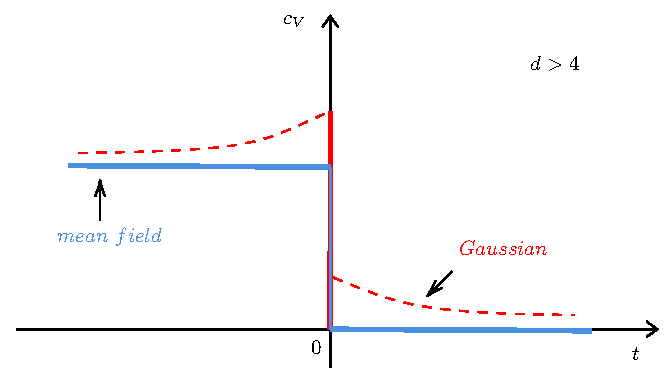
\includegraphics[width=1\textwidth]{./img/2__1.pdf}  \label{fig:18_2_1} }
\end{minipage}
\begin{minipage}[]{0.5\linewidth}
\centering
\subfloat[][Case \( d<4 \).]{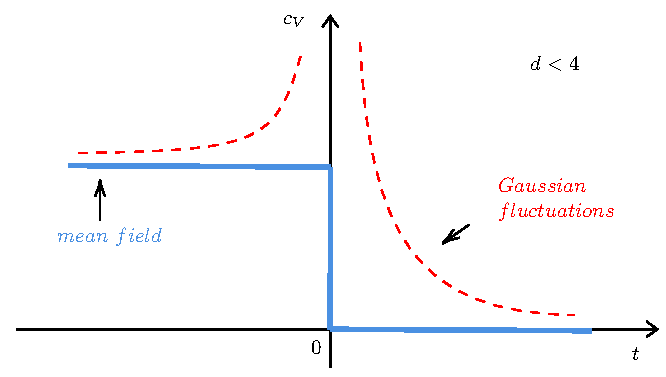
\includegraphics[width=1\textwidth]{./img/3__1.pdf}  \label{fig:18_2_2} }
\end{minipage}
\caption{\label{fig:} Behaviour of the specific heat \( c_V \) as a function of the rescaled temperature \( t \). In blue it is represented its behaviour in the mean field theory, while in red the one with Gaussian approximations. We see that in the case \( d<4 \) with Gaussian approximations the specific heat diverges near \( t \sim 0 \). }
\end{figure}




\subsubsection{Two-point correlation function in the Gaussian approximation}
We have to compute the  \( 2 \)-point correlation function for \( \mathcal{H}_{eff}^G (\varphi) \).
We know that the (simple)  correlation function is defined as:
\begin{equation*}
  G ( \va{r}, \va{r}') = \expval{ \varphi(\va{r})\varphi(\va{r}')}
\end{equation*}
so we first have to determine:
\begin{equation*}
   \varphi(\va{r})\varphi(\va{r}') = \frac{1}{V^2} \sum_{\va{k}, \va{k}'}^{}
   e^{i (\va{k} \vdot \va{r} + \va{k}' \vdot \va{r}')} \varphi_{\va{k}} \varphi_{\va{k}'}
\end{equation*}
Shifting to Fourier space, we have (the subscript \( G \) stands for Gaussian):
\begin{equation*}
  \expval{\varphi _{\va{k}} \varphi _{\va{k}'}}_G =
\frac{\int_{- \infty }^{+ \infty } \dd[]{  \varphi_{\va{k}_1} }  \dots
  \dd[]{  \varphi_{\va{k}} }  \dd[]{ \varphi_{\va{k}'} }
   \varphi_{\va{k}} \varphi_{\va{k}'} e^{- \beta \mathcal{H}_{eff}}
 }{
 \int_{- \infty }^{+ \infty } \dd[]{  \varphi_{\va{k}_1} }  \dots
   \dd[]{  \varphi_{\va{k}} }  \dd[]{ \varphi_{\va{k}'} }
    e^{- \beta \mathcal{H}_{eff}}
 }
\end{equation*}
where, as we said,
\begin{equation*}
  \mathcal{H}_{eff}^G = V A_0  + \frac{1}{2V} \sum_{\va{k}}^{} \qty(2 a t + c  \abs{\va{k}}^2) \abs{\varphi _{\va{k}}}^2
\end{equation*}
It is clear that in \(   \expval{\varphi _{\va{k}} \varphi _{\va{k}'}}_G  \)  all the integrals factorize since the Fourier modes are all independent (they are decoupled); therefore, all the integrals in the numerator that don't involve \( \va{k} \) or \( \va{k}' \) simplify with the same integrals in the denominator. Taking this into account, it is possible to show
\begin{equation*}
  \expval{\varphi _{\va{k}} \varphi _{\va{k}'}}_G =  \frac{V}{2 a t + c \abs{\va{k}}^2} \delta _{\va{k},-\va{k}'}
\end{equation*}
that, in the limit \( V \rightarrow \infty  \) (Eq.\eqref{eq:18_5}) becomes
\begin{equation}
    \expval{\varphi _{\va{k}} \varphi _{\va{k}'}}_G \overset{V \rightarrow \infty }{\longrightarrow} \frac{(2 \pi )^d}{2 a t + c \abs{\va{k}}^2} \delta  (\va{k}+ \va{k}')
\end{equation}
Going back to real space, by antitransforming, we have:
\begin{equation*}
\begin{split}
  \expval{\varphi (\va{r}) \varphi (\va{r}')}_G &= \frac{1}{V^2} \sum_{\va{k}, \va{k}'}^{} e^{i (\va{k}\vdot \va{r} + \va{k}' \vdot \va{r}' )} \expval{\varphi _{\va{k}} \varphi _{\va{k}'}}_G
  = \frac{1}{V^2} \sum_{\va{k}, \va{k}'}^{} e^{i (\va{k}\vdot \va{r} + \va{k}' \vdot \va{r}' )}   \frac{V}{2at+c\abs{\va{k}}^2} \delta _{\va{k}, -\va{k}'} \\
  & = \frac{1}{V} \sum_{\va{k}}^{} \frac{ e^{i \va{k}\vdot ( \va{r} - \va{r}' )}}{2 a t + c \abs{\va{k}}^2}
\end{split}
\end{equation*}
We see that defining:
\begin{equation*}
  \xi  (t) = \qty(\frac{c}{2at})^{1/2}
\end{equation*}
we get
\begin{equation}
    \expval{\varphi (\va{r}) \varphi (\va{r}')}_G = \frac{1}{ V } \sum_{\va{k}}^{} \frac{1}{c} \frac{ e^{i \va{k}\vdot ( \va{r} - \va{r}' )} }{ \abs{\va{k}}^2 + \xi ^{-2}}
    = \frac{1}{V} \sum_{\va{k}}^{} e^{i \va{k} \vdot \va{x}} \hat{G} (\va{k})
\end{equation}
where we have defined the correlation function
\begin{equation}
  \hat{G} (\va{k}) = \frac{1}{c} \frac{1}{   \abs{\va{k}}^2 + \xi ^{-2} }
\end{equation}
this correlation function acquires the same form of the one computed in mean field theory. This means that the critical exponents \( \nu  \) and \( \eta  \)  now have the same values predicted by mean field theory (see Sec.(\ref{sec:17_1}) and Sec.(\ref{sec:18_1})), namely:
\begin{equation}
\Rightarrow
  \begin{cases}
   \nu _{G} = \frac{1}{2}\\
   \eta_{G} = 0
  \end{cases}
\end{equation}
hence, there are no changes with Gaussian fluctuations! Interactions between \( \varphi _{\va{k}} \) are needed!


\section{Summary}

Critical exponents in the gaussian approximation
$$\gamma = 1 \quad \beta = \frac{1}{2} \quad  \delta = 3\quad \nu = \frac{1}{2}\quad  \eta = 0$$
So we get
$$\alpha = \nu(4-D) = 2 - \frac{D}{2}\quad  \text{if } D < 4$$
The gaussian approximation gives the same values of the critical exponents found within the mean field approximation where all modes of the fluctuations are neglected.
The only exception is the $\alpha$ exponent for $D < 4$. The divergence of $C$ for $D < 4$ is due to fluctuations modes with small $\mid \vec{k}\mid$, i.e. long wavelength fluctuations.
On the other hand, as $\mid t\mid \to 0$ fluctuations are very large and correlated.
To include interactions between wave modes $\varphi_{\vec{k}}$ one has to keep the quartic term $\frac{b}{2}\varphi^{4}$ in $\beta \mathcal{H}_{eff}$.



\end{document}
